\documentclass[paper=a4, fontsize=11pt]{scrartcl} % A4 paper and 11pt font size

\usepackage{float}
\usepackage{graphicx}
\usepackage{latexsym}
\usepackage{extarrows}
\usepackage[T1]{fontenc} % Use 8-bit encoding that has 256 glyphs
%\usepackage{fourier} % Use the Adobe Utopia font for the document - comment this line to return to the LaTeX default
\usepackage[english]{babel} % English language/hyphenation
\usepackage{amsmath,amsfonts,amsthm} % Math packages

\usepackage{lipsum} % Used for inserting dummy 'Lorem ipsum' text into the template

\usepackage{sectsty} % Allows customizing section commands
\allsectionsfont{\centering \normalfont\scshape} % Make all sections centered, the default font and small caps

\usepackage{fancyhdr} % Custom headers and footers
\pagestyle{fancyplain} % Makes all pages in the document conform to the custom headers and footers
\fancyhead{} % No page header - if you want one, create it in the same way as the footers below
\fancyfoot[L]{} % Empty left footer
\fancyfoot[C]{} % Empty center footer
\fancyfoot[R]{\thepage} % Page numbering for right footer
\renewcommand{\headrulewidth}{0pt} % Remove header underlines
\renewcommand{\footrulewidth}{0pt} % Remove footer underlines
\setlength{\headheight}{13.6pt} % Customize the height of the header

\numberwithin{equation}{section} % Number equations within sections (i.e. 1_1, 1_2, 2_1, 2_2 instead of 1, 2, 3, 4)
\numberwithin{figure}{section} % Number figures within sections (i.e. 1_1, 1_2, 2_1, 2_2 instead of 1, 2, 3, 4)
\numberwithin{table}{section} % Number tables within sections (i.e. 1_1, 1_2, 2_1, 2_2 instead of 1, 2, 3, 4)

\setlength\parindent{0pt} % Removes all indentation from paragraphs - comment this line for an assignment with lots of text

%----------------------------------------------------------------------------------------
%	TITLE SECTION
%----------------------------------------------------------------------------------------

\newcommand{\horrule}[1]{\rule{\linewidth}{#1}} % Create horizontal rule command with 1 argument of height

\title{	
\normalfont \normalsize 
\horrule{0.5pt} \\[0.4cm] % Thin top horizontal rule
\huge Assignment2 \\ % The assignment title
\horrule{2pt} \\[0.5cm] % Thick bottom horizontal rule
}

\author{Qinyun Song 5120309059} % Your name

\date{\normalsize\today} % Today's date or a custom date

\begin{document}

\maketitle % Print the title

%----------------------------------------------------------------------------------------
%	PROBLEM 1
%----------------------------------------------------------------------------------------
\newpage
\section*{Problem 1}
	\begin{quote}
		Consider the context-free grammar:
		\begin{displaymath}
			S \to SS+ | SS* | a
		\end{displaymath}
		and the string:
		\begin{displaymath}
			aa+a*
		\end{displaymath}
	\end{quote}
\subsection*{Leftmost derivation for the string}
	\begin{displaymath}
		S \xLongrightarrow[lm]{} SS* \xLongrightarrow[lm]{} SS+S* \xLongrightarrow[lm]{} aS+S* \xLongrightarrow[lm]{} aa+S* \xLongrightarrow[lm]{} aa+a*
	\end{displaymath}
\subsection*{Rightmost derivation for the string}
	\begin{displaymath}
		S \xLongrightarrow[rm]{} SS* \xLongrightarrow[rm]{} Sa* \xLongrightarrow[rm]{} SS+a* \xLongrightarrow[rm]{} Sa+a* \xLongrightarrow[rm]{} aa+a*
	\end{displaymath}
\subsection*{Parse tree for the string}
	\begin{figure}[H]
	\centering
	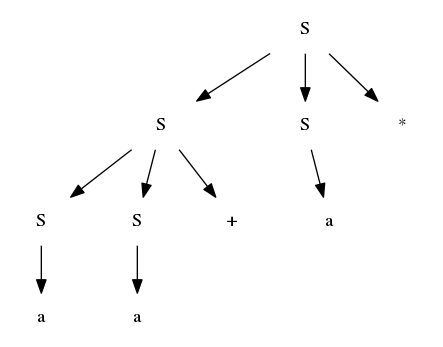
\includegraphics[width=0.5\textwidth]{parseTree.png}
	%\caption{A parse tree for the string}
	\end{figure}
%----------------------------------------------------------------------------------------
	
%----------------------------------------------------------------------------------------
%	PROBLEM 2
%----------------------------------------------------------------------------------------
\newpage
\section*{Problem 2}
\subsection*{a}
	This grammar is already left factored.
\subsection*{b}
	No.
\subsection*{c}
	\begin{eqnarray*}
		rexpr \to rterm rexpr' \\
		rexpr' \to +rterm rexpr' | \epsilon \\
		rterm \to rfactor rterm' \\
		rterm' \to rfactor rterm' | \epsilon \\
 		rfactor \to rprimary *rfactor' \\
		rfactor' \to *rfactor' | \epsilon \\
		rprimary \to a | b
	\end{eqnarray*}
\subsection*{d}
	Yes.
%----------------------------------------------------------------------------------------

%----------------------------------------------------------------------------------------
%	PROBLEM 3
%----------------------------------------------------------------------------------------
\newpage
\section*{Problem 3}
	Compute FIRST and FOLLOW for the grammar:
\subsection*{a}
	\begin{quote}
		\begin{displaymath}
			S \to 0S1 | 01withstring000111
		\end{displaymath}
	\end{quote}
	FIRST(S) = \{0\}
	
	FOLLOW(S) = \{1, \$\}
\subsection*{b}
	\begin{quote}
		\begin{displaymath}
			S \to +SS | *SS | awithstring+*aaa
		\end{displaymath}
	\end{quote}
	
	FIRST(S) = \{+, *, a\}
	
	FOLLOW(S) = \{+, *, a, \$\}
%----------------------------------------------------------------------------------------

\end{document}
